\documentclass{article}
\usepackage{graphicx}


% Title Page
\title{Systems Engineering HW 2}
\author{Caleb Groves}


\begin{document}
\maketitle

\begin{abstract}
	This is a preliminary exploration of using design of experiments (DOE) and data fitting/modeling techniques to describe and understand the relationships between successive-loop PID control of the lateral dynamics of a miniature air-vehicle (MAV). Though the DOE process shows promise in identifying possible combinations for stable performance of the aircraft, no accurate fit surrogate model could be made from the data generated by the model used.
\end{abstract}

\section{Model and Objectives}
For my model, I selected the lateral dynamics of a miniature unmanned aircraft (MAV) under successive-loop closure PID control, which I had previously developed in another course. The model’s inputs consisted of two gains for the outer loop (proportional and integral gain), and three for the inner roll-control loop (PID gains). The model uses the nonlinear dynamics and the autopilot algorithms to simulate the MAV’s response to a step-input of a 20 degree course change. From this response, it calculates the rise time, overshoot, and settling time for the MAV over a fifty-second period of simulation time.
\\\\The objective of this experiment was to see if I could understand the interactions between the five gain values and construct a predictive model for the MAV’s course rise time, overshoot, and settling time in response to a step input. Ultimately, I want to optimize these metrics to achieve superior aircraft control response.

\section{Design of Experiments (DOE)}
To achieve the objective of this experiment, I chose to use the JMP data analysis tool to generate a range of inputs for the five gain values. Since I knew that extreme values of the gains were likely to cause unstable responses, I selected a Latin Hypercube Space Filling design to try to span and cover the interior areas of the design space as best as possible. The five gain values were modeled as continuous, which is perfectly feasible since digital controllers can use any gain value the design wants.
\\\\I initially did a run of five hundred points with a very wide range of gain values, which quickly showed me that most of the design space (95\%) that I had chosen gave unstable system responses. After narrowing down the design space to values between zero and three for the proportional gains, zero to one for the integral gains, and zero to two for the derivative gains, I had a much more interesting design space to work in. The final DOE contained five thousand points, and took over five hours to run.

\section{Surrogate Model and Evaluation}
Though I tried many different possible factor combinations and fits, I could not find any satisfactory surrogate model for this experiment. Even using third or fourth degree polynomial models, R-squared values usually flat-lined at around 0.6.
\\\\Though some of this might be poor analysis techniques or a lack of understanding about model-fitting on my end, a large of part of this may also be a problem with the model that is being used and the metrics used to evaluate it.

\subsection{Best Fit Model}
Unfortunately, I have run out of time to even include any graphs or any of the very long and nasty fit equations that account for so little of the behavior of this system. In the last five minutes I've decided to try and at least give you this (some of the fit equation for rise-time):
\\\\
$t_r = 1.779 - 0.1352 kp_{\chi} - 0.362 ki_{\chi} + 0.037 kp_{\phi} + 0.163 kd_{\phi} + (kp_{\chi} - 1.749) ((ki_{\chi} - 0.814) 0.186) $

\begin{figure}
	\centering
	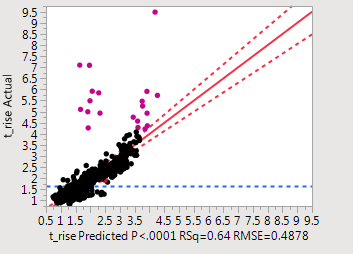
\includegraphics[scale=0.5]{t_rise_actual_vs_predicted.png}
	\caption{Actual vs. predicted plot from JMP using a 4th order fit. Unfortunately, I could find no compelling justification for excluding the outliers (purple points) based on observing these points' overshoot and settling time.}
\end{figure}


\subsection{Model Flaws}
Unstable system responses give a settling time of infinity, which just ends up being written out as a non-numerical output. In retrospect, I'm not sure if I dealt with this issue very well, since I changed it from Matlab's "NaN" (\textit{Not a Number}) to 100 so that JMP could read it, since 100 is far beyond the 50 second simulation time and would be easy to identify as an unstable response. This adds a very nonlinear dynamic to the output trends. Since it was very nonsensical to try and interpret these unstable responses, I tried removing them from the analysis, but even this bit of cheating did little to help find a more suitable surrogate model fit.
\\\\Another limitation was the simulation time itself, which I limited to fifty seconds. This may have truncated some system responses which otherwise would have converged; the only way to tell would be to run the same set of inputs with a longer simulation time and compare the number of infinite settling times recorded.
\\\\Finally, another weakness of the model was that although rise time, settling time, and overshoot are fairly good metrics for evaluating a system's response, they are not totally sufficient for describing the aircraft's stability in this case. There can be a kind of "control noise", where low overshoot, fast rise time, and quick settling time are attained, but the aircraft is controlled using high frequency correction commands. This is undesirable, and the current three outputs have no way of identifying or describing this. I discovered this by using some promising outputs from the DOE in my MAV simulator developed for ME EN 634 (Flight Dynamics and Controls). Developing another output or outputs that can describe the "noisiness" of the system's response could help to more fully define the kinds of responses we want (perhaps by doing a discrete Fourier analysis on the course output).
\\\\A similar system response that warrants its own output and evaluation is the total roll angle during the course-correction maneuver. I observed that sometimes good rise time, overshoot, and settling time were achieved with a certain gain combination, but the MAV performed its course-correction by barrel-rolling several times before settling into a good flight path. Though this seems to work well enough in the simulation, I expect this to be a less-desirable in-flight behavior for most situations.

\section{Conclusions}
As I am writing this, this is two minutes late, so I will sum up: I think this was an excellent exercise and could be a really good project. Unfortunately, I was not able to find a good model fit yet, possibly due to the model I was using but also because I didn't go get help with these problems sooner. I hope I have demonstrated an understanding of the overall process, if not the specific tools of JMP and data analysis yet. Hopefully you will have mercy on me in this assignment since I didn't have much to do analysis and metrics on (well, I guess I could have shown bad metrics, I was just too focused on trying to get to where I could show good metrics).


\end{document}          
